\documentclass[A4,svgnames,9pt,aspectratio=169]{beamer}
%% document options:
%% - aspectratio = { 43, 169, 1610 }
%% - utf8

\usepackage{amsmath,amssymb,amsfonts,amsthm,mathtools}
\usepackage{tikz}
\usepackage{booktabs}
\usepackage[backend=bibtex,style=numeric,sorting=none]{biblatex}

% Add bibliography resource
\addbibresource{referencesThesis.bib}

% TikZ Libraries
\usetikzlibrary{fit,backgrounds,shapes.geometric,patterns,decorations.pathreplacing,positioning,arrows.meta}

% Custom TikZ styles from ChapII.tex
\tikzset{
  chapbox/.style={draw,rounded corners,very thick,align=center,fill=gray!8,inner sep=5pt,minimum height=1.05cm},
  chapboxdark/.style={draw,rounded corners,very thick,align=center,fill=gray!18,inner sep=5pt,minimum height=1.05cm},
  chaparr/.style={-{Latex[length=2.4mm]},very thick},
  chapdash/.style={-{Latex[length=2.4mm]},very thick,dashed},
  spin/.style={circle,draw,inner sep=0pt,minimum size=5mm,font=\scriptsize,fill=white},
  tinynode/.style={circle,draw,inner sep=0pt,minimum size=3.8mm,font=\tiny,fill=white},
  posedge/.style={line width=1pt},
  negedge/.style={line width=1pt,dashed},
  freeze/.style={line width=1.6pt},
  faint/.style={line width=.45pt,gray!55},
  triwhite/.style={draw,fill=gray!8,line width=.6pt},
  trigray/.style={draw,fill=gray!22,line width=.6pt},
  % Local styles for haplotype figure
  read/.style={line width=5pt, gray!45, line cap=round, preaction={draw, white, line width=7pt, line cap=round}},
  readlink/.style={densely dotted, thick, gray!60},
  errlabel/.style={font=\scriptsize\bfseries, text=red!80!black, fill=white, inner sep=1.5pt, rounded corners=2pt},
  interedge/.style={negedge, draw=gray!60}
}

% Triangular Icon macros from ChapII.tex
\newcommand{\ChapTriangleIcon}[2][1.65ex]{%
  \begingroup
  \pgfmathsetlengthmacro{\TriangleH}{#1}%
  \tikz[
    baseline=-0.25ex,
    x=\TriangleH,
    y=\TriangleH,
    line cap=round,
    line join=round
  ]{%
    \path[use as bounding box]
      (-0.08,-0.12) rectangle (1.24,1.12);
    \draw[#2]
      (0,0)
      --
      (1.1547,0)
      --
      (0.57735,1)
      --
      cycle;
  }%
  \endgroup
}

\DeclareRobustCommand{\TriangleAttractif}[1][2.5ex]{%
  \ChapTriangleIcon[#1]{posedge}%
}

\DeclareRobustCommand{\TriangleRepulsif}[1][2.5ex]{%
  \ChapTriangleIcon[#1]{negedge}%
}

% General macros
\newcommand{\SB}{\textsc{Sankararaman}--\textsc{Baccelli}}
\newcommand{\ov}{\operatorname{ov}}
\newcommand{\Conf}{\mathcal{C}}
\newcommand{\Lab}{\mathcal{L}}
\newcommand{\Obs}{\mathcal{O}}
\newcommand{\ind}[1]{\mathbb{I}_{\{#1\}}}

\newcommand{\drawHaplotypePresentation}[1]{%
  \begin{tikzpicture}[scale=0.74, x=1.0cm, y=1.2cm, font=\footnotesize]
    % 1. CHROMOSOME LINES (GROUND TRUTH)
    \draw[faint, dashed] (-1.5, 3.5) -- (13.5, 3.5) node[right, text=black, align=left] {\textbf{Haplotype 1}\\(Truth {\Large $\boldsymbol{\Sigma}$} $= +$)};
    \draw[faint, dashed] (-1.5, 0) -- (13.5, 0) node[right, text=black, align=left] {\textbf{Haplotype 2}\\(Truth {\Large $\boldsymbol{\Sigma}$} $= -$)};

    % 2. BACKGROUND: READS AND SEGMENTS (step >= 2)
    \ifnum#1>1\relax
      \begin{scope}[on background layer]
        % --- Reads (Segments) ---
        \draw[readlink] (1, 3.5) -- (1, 4.0); \draw[read] (-1.2, 4.0) -- (3.2, 4.0); 
        \draw[readlink] (3, 3.5) -- (3, 4.4); \draw[read] (0.8, 4.4) -- (5.2, 4.4); 
        \draw[readlink] (5, 3.5) -- (5, 4.8); \draw[read] (2.8, 4.8) -- (7.2, 4.8); 
        \draw[readlink] (7, 3.5) -- (7, 4.0); \draw[read] (4.8, 4.0) -- (9.2, 4.0); 
        \draw[readlink] (9, 3.5) -- (9, 4.4); \draw[read] (6.8, 4.4) -- (11.2, 4.4); 
        \draw[readlink] (11, 3.5) -- (11, 4.8); \draw[read] (8.8, 4.8) -- (13.2, 4.8); 

        % Haplotype 2
        \draw[readlink] (2, 0) -- (2, 0.5); \draw[read] (-0.2, 0.5) -- (4.2, 0.5); 
        \draw[readlink] (4, 0) -- (4, 0.9); \draw[read] (1.8, 0.9) -- (6.2, 0.9); 
        \draw[readlink] (6, 0) -- (6, 1.3); \draw[read] (3.8, 1.3) -- (8.2, 1.3); 
        \draw[readlink] (8, 0) -- (8, 0.5); \draw[read] (5.8, 0.5) -- (10.2, 0.5); 
        \draw[readlink] (10, 0) -- (10, 0.9); \draw[read] (7.8, 0.9) -- (12.2, 0.9); 
        \draw[readlink] (12, 0) -- (12, 1.3); \draw[read] (9.8, 1.3) -- (14.2, 1.3); 
      \end{scope}

      % NODES (SPIN CENTERS) - Now visible starting from step 2!
      \node[spin, fill=gray!8] (t1) at (1, 3.5) {$+$};
      \node[spin, fill=gray!8] (t2) at (3, 3.5) {$+$};
      \node[spin, fill=gray!8] (t3) at (5, 3.5) {$+$};
      \node[spin, fill=gray!8] (t4) at (7, 3.5) {$+$};
      \node[spin, fill=gray!8] (t5) at (9, 3.5) {$+$};
      \node[spin, fill=gray!8] (t6) at (11, 3.5) {$+$};

      \node[spin, fill=gray!20] (b1) at (2, 0) {$-$};
      \node[spin, fill=gray!20] (b2) at (4, 0) {$-$};
      \node[spin, fill=gray!20] (b3) at (6, 0) {$-$};
      \node[spin, fill=gray!20] (b4) at (8, 0) {$-$};
      \node[spin, fill=gray!20] (b5) at (10, 0) {$-$};
      \node[spin, fill=gray!20] (b6) at (12, 0) {$-$};
    \fi

    % 3. SIGNED GRAPH EDGES ONLY (step >= 3)
    \ifnum#1>2\relax
      \begin{scope}[on background layer]
        % --- Inter-Chromosome Edges (True Negatives) ---
        \draw[interedge] (1, 3.5) -- (2, 0); 
        \draw[interedge] (3, 3.5) -- (4, 0); 
        \draw[interedge] (3, 3.5) -- (6, 0); 
        \draw[interedge] (5, 3.5) -- (2, 0); 
        \draw[interedge] (5, 3.5) -- (4, 0); 
        \draw[interedge] (5, 3.5) -- (6, 0); 
        \draw[interedge] (7, 3.5) -- (4, 0); 
        \draw[interedge] (7, 3.5) -- (6, 0); 
        \draw[interedge] (7, 3.5) -- (8, 0); 
        \draw[interedge] (7, 3.5) -- (10, 0); 
        \draw[interedge] (9, 3.5) -- (8, 0); 
        \draw[interedge] (9, 3.5) -- (10, 0); 
        \draw[interedge] (9, 3.5) -- (12, 0); 
        \draw[interedge] (11, 3.5) -- (8, 0); 
        \draw[interedge] (11, 3.5) -- (12, 0); 

        % False Positives (FP) => 25% noise
        \draw[posedge, draw=red!80!black] (1, 3.5) -- node[errlabel, pos=0.2] {FP} (4, 0); 
        \draw[posedge, draw=red!80!black] (3, 3.5) -- node[errlabel, pos=0.8] {FP} (2, 0); 
        \draw[posedge, draw=red!80!black] (5, 3.5) -- node[errlabel, pos=0.2] {FP} (8, 0); 
        \draw[posedge, draw=red!80!black] (9, 3.5) -- node[errlabel, pos=0.8] {FP} (6, 0); 
        \draw[posedge, draw=red!80!black] (11, 3.5) -- node[errlabel, pos=0.2] {FP} (10, 0); 
      \end{scope}

      % INTRA-EDGES
      \draw[posedge] (t1) to[bend right=25] (t2);
      \draw[negedge, draw=red!80!black] (t2) to[bend right=25] node[errlabel] {FN} (t3);
      \draw[posedge] (t3) to[bend right=25] (t4);
      \draw[posedge] (t4) to[bend right=25] (t5);
      \draw[posedge] (t5) to[bend right=25] (t6);
      
      \draw[posedge] (t1) to[bend right=35] (t3);
      \draw[posedge] (t2) to[bend right=35] (t4);
      \draw[negedge, draw=red!80!black] (t3) to[bend right=35] node[errlabel] {FN} (t5);
      \draw[posedge] (t4) to[bend right=35] (t6);

      \draw[posedge] (b1) to[bend right=25] (b2);
      \draw[posedge] (b2) to[bend right=25] (b3);
      \draw[posedge] (b3) to[bend right=25] (b4);
      \draw[negedge, draw=red!80!black] (b4) to[bend right=25] node[errlabel] {FN} (b5);
      \draw[posedge] (b5) to[bend right=25] (b6);
      
      \draw[negedge, draw=red!80!black] (b1) to[bend right=35] node[errlabel] {FN} (b3);
      \draw[negedge, draw=red!80!black] (b2) to[bend right=35] node[errlabel] {FN} (b4);
      \draw[posedge] (b3) to[bend right=35] (b5);
      \draw[posedge] (b4) to[bend right=35] (b6);
    \fi

    % 5. LEGEND
    \ifnum#1=2\relax
      \node[scale=0.65,chapbox, align=left, fill=white] at (0,1.75){
        \begin{tabular}{ll}
          \tikz[baseline=-0.5ex]{\draw[line width=5pt, gray!45, line cap=round] (0,0) -- (0.6,0);} & DNA Read (Segment) \\
          \tikz[baseline=-0.5ex]{\node[spin, scale=0.6, fill=gray!8] at (0,0) {$+$};} & Graph Node (true assignment {\Large $\boldsymbol{\Sigma}$})
        \end{tabular}
      };
    \fi
    \ifnum#1>2\relax
      \node[scale=0.65,chapbox, align=left, fill=white] at (0,1.75){
        \begin{tabular}{ll}
          \tikz[baseline=-0.5ex]{\draw[line width=5pt, gray!45, line cap=round] (0,0) -- (0.6,0);} & DNA Read (Node) \\
          \tikz[baseline=-0.5ex]{\draw[posedge] (0,0) -- (0.6,0);} & Attraction (solid line)  \\
          \tikz[baseline=-0.5ex]{\draw[negedge] (0,0) -- (0.6,0);} & Repulsion (dashed line) \\
          \textcolor{red!80!black}{\textbf{FP}} & False Positive (noise)  \\
          \textcolor{red!80!black}{\textbf{FN}} & False Negative (noise)
        \end{tabular}
      };
    \fi
  \end{tikzpicture}
}

\hypersetup{
   allcolors=rouge_inria,
   pdfauthor   = {Louis Hauseux},
   pdftitle    = {Community Detection on Signed Graphs},
   pdfsubject  = {Seminar of the MathNet team (Inria Paris)},
   pdfkeywords = {community detection, signed graphs, MCMC, Swendsen-Wang, coupling}
}

\title[Community Detection on Signed Graphs]{Community Detection on Signed Graphs:\\A Bayesian MCMC Coupling Approach}
\subtitle{Seminar of the MathNet team (Inria Paris)}
\institute{Inria Paris, Room Paul \textsc{Erdös} (A115) -- 2 p.m.}
\date[15 June 2026]{Monday 15 June 2026}
\author[L. Hauseux]{\href{https://team.inria.fr/neo/author/louis-hauseux/}{Louis \textsc{Hauseux}} {\small(Inria Sophia Antipolis, superv. by \href{https://www-sop.inria.fr/members/Konstantin.Avratchenkov/}{K. \textsc{Avrachenkov}} \& \href{https://www-sop.inria.fr/members/Josiane.Zerubia/index-eng.html}{J. \textsc{Zerubia}})}\\[3pt]
{\small Joint work with \href{https://nahuelsopranoloto.github.io/}{Nahuel \textsc{Soprano-Loto}} (Inria Paris)}\\
{\small and \href{https://www-sop.inria.fr/members/Konstantin.Avratchenkov/}{Konstantin \textsc{Avrachenkov}} (Inria Sophia Antipolis)}}

\usetheme{inria}

\begin{document}

\frame{\titlepage}

\renewcommand{\contentsname}{Outline}
\frame{\tocpage}

%%%%%%%%%%%%%%%%%%%%%%%%%%%%%%%%%%%%%%%%%%%%%%%%%%%%%%%
\section{Motivation \& the \textsc{Sankararaman}--\textsc{Baccelli} Model}
\frame{\sectionpage}

\begin{frame}{Haplotype Assembly}
  \centering
  \only<1>{%
    \begin{block}{1. Biological Setup: Two Homologous Chromosomes (Haplotypes)}
      Humans are diploid: they have two copies of each chromosome (homologous chromosomes).
    \end{block}
    \drawHaplotypePresentation{1}
  }%
  \only<2>{%
    \begin{block}{2. High-Throughput Sequencing: DNA Reads}
      Sequencing generates short, overlapping fragments called \textbf{reads} from both chromosomes.
    \end{block}
    \drawHaplotypePresentation{2}
  }%
  \only<3>{%
    \begin{block}{3. Modeling as a Signed Graph}
      Nodes = reads \qquad Edges = overlaps\\
      \textbf{Goal:} Reconstruct the true haplotype assignments {\Large $\boldsymbol{\Sigma}$} from this observed signed graph.
    \end{block}
    \drawHaplotypePresentation{3}
  }%
\end{frame}

\begin{frame}{Motivation: Signed Community Detection}
  \begin{block}{Community Detection on Signed Graphs ($K=2$)}
    \begin{itemize}
      \item We aim to partition nodes into $K=2$ communities: {\Large $\boldsymbol{\Sigma}_i$} $\in \{+1, -1\}$.
      \item Observed links represent \textbf{attractions} (solid lines) and \textbf{repulsions} (dashed lines).
      \item Under the hood, this is a \textbf{Stochastic Block Model} (SBM) setup.
    \end{itemize}
  \end{block}
  \begin{block}{The Geometric Challenge}
    \begin{itemize}
      \item Nodes are embedded in space (e.g., genomic positions on $\mathbb{Z}$ or $\mathbb{R}^d$).
      \item Edge probabilities depend directly on the distance $r = \|x_i - x_j\|$:
        \begin{align*}
            \mathbb{P}(\text{attractive edge} \mid \text{same community}) &= f_{\mathrm{in}}(r) \\
            \mathbb{P}(\text{repulsive edge} \mid \text{different communities}) &= f_{\mathrm{out}}(r)
        \end{align*}
      \item \textbf{All the difficulty (and the interest!) comes from this geometric dependency.}
    \end{itemize}
  \end{block}
\end{frame}

\begin{frame}{The \textsc{Sankararaman}--\textsc{Baccelli} Model (GSBM)}
  \begin{block}{Model Definition \cite{SankararamanBaccelli2018}}
    \begin{itemize}
      \item \textbf{Spatial Nodes $V_n$}: Hom. \textsc{Poisson} PP $\mathcal{X}$ in $\mathbb{R}^d$ \cite{BB} restrict. to a $n$-volume window.
      \item \textbf{Latent Communities}: Uniform assignments $\Sigma_i \in \{+1, -1\}$ ($K=2$).
      \item \textbf{Geometric Overlaps}: Observed connection $e=\{i,j\} \in H$ with probability:
        \begin{equation*}
            \mathbb{P}(e \in H \mid X, \Sigma) =
            \begin{cases}
                f_{\mathrm{in}}(r_e) & \text{if } \Sigma_i = \Sigma_j \text{ (attraction),} \\
                f_{\mathrm{out}}(r_e) & \text{if } \Sigma_i \neq \Sigma_j \text{ (repulsion),}
            \end{cases}
        \end{equation*}
        with distance $r_e = \|X_i - X_j\|$ and connecting functions $f_{\mathrm{in}}(r) \ge f_{\mathrm{out}}(r)$.
    \end{itemize}
  \end{block}
  \begin{block}{Goal: Weak Recovery}
    \begin{itemize}
      \item Find an algorithm $\tau$ (independent of $\Sigma$) reconstructing assignments:
        \begin{equation*}
            \lim_{n\to\infty} \mathbb{E}[\ov_n(\Sigma, \tau)] \ge \frac{1}{2} + \eta \quad \text{for some } \eta > 0,
        \end{equation*}
        using the \textbf{Community Overlap}: $\ov_n(\Sigma, \tau) = \max_{\pi \in \mathfrak{S}_2} \frac{1}{n} \sum_{i=1}^n \ind{\tau_i = \pi(\Sigma_i)}$.
    \end{itemize}
  \end{block}
\end{frame}

\begin{frame}{Gibbs Model on Signed Graphs}
  \begin{block}{Signed Interaction Graph}
    \begin{itemize}
      \item Let $E$ be the set of potential edges. Each edge $e=\{i,j\}$ has a weight $W_e \in \mathbb{R}$.
      \item $W_e > 0$ represents an \textbf{attraction} (tending to align community labels: $\sigma_i = \sigma_j$).
      \item $W_e < 0$ represents a \textbf{repulsion} (tending to separate community labels: $\sigma_i \neq \sigma_j$).
    \end{itemize}
  \end{block}
  \begin{block}{Signed Gibbs Measure}
    \begin{itemize}
      \item The probability of a label configuration $\sigma \in \{+1, -1\}^{V_n}$ is given by:
        \begin{equation*}
            \mu(\sigma) = \frac{1}{Z} e^{-U(\sigma)} = \frac{1}{Z} \exp\left(-\sum_{e=\{i,j\}\in E} \psi_{W_e}(\sigma_i,\sigma_j)\right)
        \end{equation*}
      \item The \textbf{local interaction potential} $\psi_w(a,b)$ penalizes unsatisfied edges:
        \begin{equation*}
            \psi_w(a,b) =
            \begin{cases}
                |w|\,\ind{a \neq b} & \text{if } w > 0 \quad \text{(penalizes different labels),} \\[1.5ex]
                |w|\,\ind{a = b} & \text{if } w < 0 \quad \text{(penalizes equal labels),} \\[1.5ex]
                0 & \text{if } w = 0.
            \end{cases}
        \end{equation*}
        The magnitude $|w|$ measures the constraint's strength.
    \end{itemize}
  \end{block}
\end{frame}

\begin{frame}{From GSBM to the Gibbs Posterior}
  \begin{block}{Conditioning on the Point Cloud}
    \begin{itemize}
      \item Once the spatial positions $X$ are observed and fixed, all pairwise distances $r_e = \|X_i - X_j\|$ are known.
      \item Under a uniform prior on $\Sigma$, the posterior distribution given the observed graph $H$ is:
        \begin{equation*}
            \mathbb{P}(\Sigma = \sigma \mid H, X) \propto \mathbb{P}(H \mid X, \sigma)
        \end{equation*}
    \end{itemize}
  \end{block}
  \begin{block}{Log-Likelihood as Signed Gibbs Energy}
    \begin{itemize}
      \item Factorizing the likelihood over all potential edges $e=\{i,j\} \in E$:
        \begin{equation*}
            \mathbb{P}(H \mid X, \sigma) \propto \exp\left(-\sum_{e\in E} \psi_{W_e(H)}(\sigma_i,\sigma_j)\right)
        \end{equation*}
      \item The posterior $\mathbb{P}(\Sigma \mid H, X)$ is exactly a \textbf{Signed \textsc{Gibbs} measure} with weights:
        \begin{equation*}
            W_e(H)=
            \begin{cases}
                \displaystyle \log\left(\frac{f_{\mathrm{in}}(r_e)}{f_{\mathrm{out}}(r_e)}\right) > 0 & \text{if } e\in H \text{ (observed overlap / attraction),}\\[2ex]
                \displaystyle -\log\left(\frac{1-f_{\mathrm{out}}(r_e)}{1-f_{\mathrm{in}}(r_e)}\right) < 0 & \text{if } e\notin H \text{ (absent overlap / repulsion).}
            \end{cases}
        \end{equation*}
    \end{itemize}
  \end{block}
\end{frame}

\begin{frame}{The Percolation Obstruction}
  \begin{block}{Necessary Condition for Weak Recovery \cite{SankararamanBaccelli2018}}
    \begin{itemize}
      \item Intuitively, if the graph is composed of many tiny, isolated components, no global community structure can be reconstructed.
      \item Information can only flow globally if the graph \textbf{percolates} (possesses a giant/infinite component).
    \end{itemize}
  \end{block}
  \begin{theorem}[\textsc{Sankararaman} \& \textsc{Baccelli} \cite{SankararamanBaccelli2018}]
    Percolation of the graph with edge probability
    \begin{equation*}
        p_e = f_{\mathrm{in}}(r_e) - f_{\mathrm{out}}(r_e)
    \end{equation*}
    is a \textbf{necessary condition} for weak recovery. If this independent bond percolation does not yield a giant component, weak recovery is mathematically impossible.
  \end{theorem}
  \begin{itemize}
    \item Our goal: Retrieve and extend this result using a unified \textbf{Bayesian MCMC coupling} framework.
  \end{itemize}
\end{frame}

%%%%%%%%%%%%%%%%%%%%%%%%%%%%%%%%%%%%%%%%%%%%%%%%%%%%%%%
\section{The Bayesian Framework \& Coupling}
\frame{\sectionpage}

\begin{frame}{The General Bayesian Model}
  \begin{definition}{General Bayesian Community Detection Model}
    \begin{enumerate}
      \item \textbf{Features}: $X_n \in \mathcal{X}_n$ with distribution $\nu_n$.
      \item \textbf{Prior}: $\mu_{0,n}(\mathrm{d}\sigma \mid x)$ over $\Conf_n = \Lab_K^{V_n}$.
      \item \textbf{Channel}: $Q_n(\mathrm{d}w \mid x, \sigma) = \prod_{e \in E_n} Q_{e,n}(\mathrm{d}w_e \mid x_i, x_j, \sigma_i, \sigma_j)$.
    \end{enumerate}
    The joint law is $\mathbb{P}_n(\mathrm{d}x, \mathrm{d}\sigma, \mathrm{d}w) = \nu_n(\mathrm{d}x)\mu_{0,n}(\mathrm{d}\sigma \mid x)Q_n(\mathrm{d}w \mid x, \sigma)$.
  \end{definition}

  \begin{figure}[H]
    \centering
    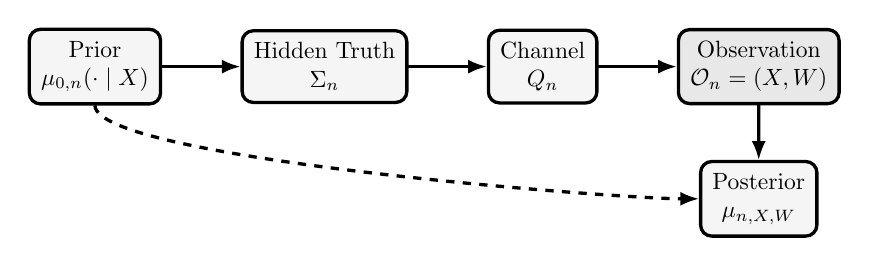
\begin{tikzpicture}[node distance=0.8cm and 1cm, scale=0.85, every node/.style={scale=0.85}]
      \node[chapbox] (prior) {Prior\\$\mu_{0,n}(\cdot\mid X)$};
      \node[chapbox,right=of prior] (truth) {Hidden Truth\\$\Sigma_n$};
      \node[chapbox,right=of truth] (chan) {Channel\\$Q_n$};
      \node[chapboxdark,right=of chan] (obs) {Observation\\$\Obs_n=(X,W)$};
      \node[chapbox,below=0.7cm of obs] (post) {Posterior\\$\mu_{n,X,W}$};
      \draw[chaparr] (prior) -- (truth);
      \draw[chaparr] (truth) -- (chan);
      \draw[chaparr] (chan) -- (obs);
      \draw[chaparr] (obs) -- (post);
      \draw[chapdash] (prior.south) .. controls +(0,-0.8) and +(-1.2,0) .. (post.west);
    \end{tikzpicture}
  \end{figure}
\end{frame}

\begin{frame}{Posterior Resampling (\textsc{Nishimori} Identity)}
  \begin{block}{Replacing Truth by a Replica}
    \begin{itemize}
      \item Since $\Sigma_n$ is hidden, we cannot compute the overlap $\ov_n(\Sigma_n, \tau_n)$ directly in an algorithm.
      \item However, under the true model, the hidden truth and a sample from the posterior are exchangeable.
    \end{itemize}
  \end{block}
  \begin{theorem}[Posterior Resampling / \textsc{Nishimori} Identity \cite{Nishimori1980}]
    Let $\tau_n$ be any community detection algorithm. Let $\Sigma_n^{(1)} \sim \mu_{n, X_n, W_n}$ be a replica drawn independently from the posterior. For any bounded test function $\Psi_n$:
    \begin{equation*}
        \mathbb{E}\left[\Psi_n(X_n, W_n, \Sigma_n, \tau_n)\right]
        =
        \mathbb{E}\left[\Psi_n(X_n, W_n, \Sigma_n^{(1)}, \tau_n)\right].
    \end{equation*}
  \end{theorem}
  \begin{corollary}{Overlap Identity}
    For any algorithm $\tau_n$ and threshold $s \in [0,1]$:
    \begin{equation*}
        \mathbb{P}\left[\ov_n(\Sigma_n, \tau_n) \ge s\right]
        =
        \mathbb{P}\left[\ov_n(\Sigma_n^{(1)}, \tau_n) \ge s\right].
    \end{equation*}
  \end{corollary}
\end{frame}

\begin{frame}{Invariant Coupling}
  \begin{block}{\textsc{Markov} Chain Dynamics as a Source of Coupling}
    \begin{itemize}
      \item To study the overlap, we need a way to construct the posterior replica $\Sigma^{(1)}$ starting from the ground truth $\Sigma$.
      \item Let $M_{n, x, w}$ be a \textsc{Markov} transition kernel that leaves the posterior $\mu_{n, x, w}$ invariant.
      \item If we initialize the chain at the hidden truth $\Sigma$, and perform \textbf{exactly one step} of the dynamics to obtain $\Sigma^{(1)} \sim M_{n, X, W}(\Sigma, \cdot)$, then $\Sigma^{(1)}$ is still distributed according to the posterior!
    \end{itemize}
  \end{block}
  \begin{figure}[H]
    \centering
    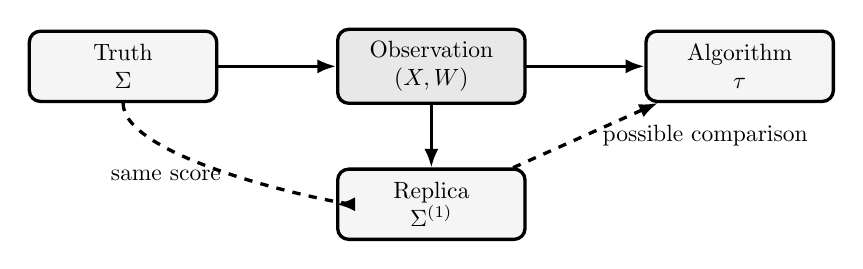
\begin{tikzpicture}[node distance=0.8cm and 1.5cm, scale=0.85, every node/.style={scale=0.85}]
      \node[chapboxdark,minimum width=2.8cm] (obs) {Observation\\$(X,W)$};
      \node[chapbox,minimum width=2.8cm,left=of obs] (true) {Truth\\$\Sigma$};
      \node[chapbox,minimum width=2.8cm,right=of obs] (algo) {Algorithm\\$\tau$};
      \node[chapbox,minimum width=2.8cm,below=of obs] (rep) {Replica\\$\Sigma^{(1)}$};
      \draw[chaparr] (true) -- (obs);
      \draw[chaparr] (obs) -- (algo);
      \draw[chaparr] (obs) -- (rep);
      \draw[chapdash] (true) .. controls +(0,-1.4) and +(-1.4,0) .. node[left]{same score} (rep);
      \draw[chapdash] (rep) -- node[right]{\ possible comparison} (algo);
    \end{tikzpicture}
  \end{figure}
\end{frame}

%%%%%%%%%%%%%%%%%%%%%%%%%%%%%%%%%%%%%%%%%%%%%%%%%%%%%%%
\section{MCMC Dynamics \& Performance Bounds}
\frame{\sectionpage}

\begin{frame}{MCMC Dynamics for Signed \textsc{Gibbs} Measures}
  \begin{block}{1. Single-Spin Dynamics (\textsc{Glauber} / \textsc{Metropolis}--\textsc{Hastings})}
    \begin{itemize}
      \item Select a node at random and update its label according to its local neighbors.
      \item Extremely slow in the presence of frustration: local updates cannot cross energy barriers.
    \end{itemize}
  \end{block}
  \begin{block}{2. \textsc{Swendsen}--\textsc{Wang} (SW) Signed Cluster Dynamics \cite{SwendsenWang, EdwardsSokal}}
    \begin{itemize}
      \item Update whole clusters of vertices simultaneously to speed up mixing.
      \item \textbf{Freezing Step}: For each edge $e=\{i,j\}$:
        \begin{itemize}
          \item If $e$ is satisfied ($W_e > 0$ and $\sigma_i = \sigma_j$, or $W_e < 0$ and $\sigma_i \neq \sigma_j$), freeze it with probability:
            \begin{equation*}
                p_e^{\mathrm{gel}} = 1 - e^{-|W_e|}.
            \end{equation*}
          \item If $e$ is unsatisfied, do not freeze it ($p_e^{\mathrm{gel}} = 0$).
        \end{itemize}
      \item \textbf{Recoloring Step}: Flip each frozen cluster independently with probability $1/2$.
    \end{itemize}
  \end{block}
\end{frame}

\begin{frame}{One Step of Signed \textsc{Swendsen}--\textsc{Wang}}
  \begin{figure}[H]
    \centering
    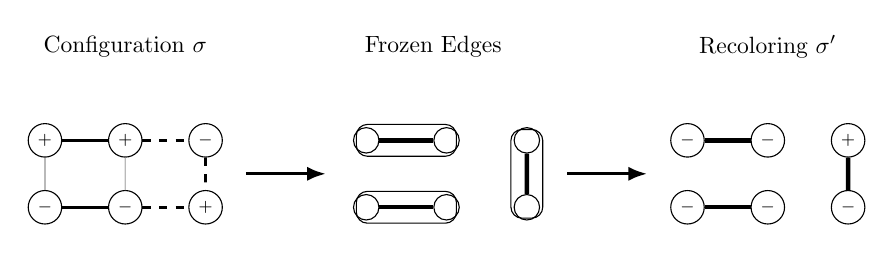
\begin{tikzpicture}[x=1cm,y=1cm, scale=0.85, every node/.style={scale=0.85}]
      \node at (1.2,2.4) {Configuration $\sigma$};
      \foreach \n/\x/\y/\s in {a/0/1/+,b/1.2/1/+,c/2.4/1/-,d/0/0/-,e/1.2/0/-,f/2.4/0/+}
        \node[spin] (\n) at (\x,\y) {$\s$};
      \draw[posedge] (a)--(b);
      \draw[negedge] (b)--(c);
      \draw[posedge] (d)--(e);
      \draw[negedge] (e)--(f);
      \draw[faint] (a)--(d); \draw[faint] (b)--(e); \draw[negedge] (c)--(f);

      \draw[chaparr] (3.0,.5)--(4.2,.5);
      \node at (5.8,2.4) {Frozen Edges};
      \foreach \n/\x/\y in {a2/4.8/1,b2/6/1,c2/7.2/1,d2/4.8/0,e2/6/0,f2/7.2/0}
        \node[tinynode] (\n) at (\x,\y) {};
      \draw[freeze] (a2)--(b2); \draw[freeze] (d2)--(e2); \draw[freeze] (c2)--(f2);
      \node[draw,rounded corners,fit=(a2)(b2),inner sep=2pt] {};
      \node[draw,rounded corners,fit=(d2)(e2),inner sep=2pt] {};
      \node[draw,rounded corners,fit=(c2)(f2),inner sep=2pt] {};

      \draw[chaparr] (7.8,.5)--(9.0,.5);
      \node at (10.8,2.4) {Recoloring $\sigma'$};
      \foreach \n/\x/\y/\s in {a3/9.6/1/-,b3/10.8/1/-,c3/12/1/+,d3/9.6/0/-,e3/10.8/0/-,f3/12/0/-}
        \node[spin] (\n) at (\x,\y) {$\s$};
      \draw[freeze] (a3)--(b3); \draw[freeze] (d3)--(e3); \draw[freeze] (c3)--(f3);
    \end{tikzpicture}
  \end{figure}
  \begin{itemize}
    \item Edges in bold represent satisfied interactions that are randomly frozen.
    \item Clusters are then flipped independently.
  \end{itemize}
\end{frame}

\begin{frame}{Coupling \& the \textsc{Sankararaman}--\textsc{Baccelli} Bound}
  \begin{block}{Gel Probability under the Generative Model}
    Let's run one step of SW starting from the hidden truth $\Sigma$. What is the probability that an edge $e$ is frozen?
    \begin{itemize}
      \item \textbf{Case 1: $\Sigma_i = \Sigma_j$}. Edge is present with probability $f_{\mathrm{in}}(r_e)$, and has weight $W_e = \log(f_{\mathrm{in}}/f_{\mathrm{out}}) > 0$.
        \begin{equation*}
            \mathbb{P}(\text{frozen}) = f_{\mathrm{in}}(r_e) \left(1 - e^{-|W_e|}\right) = f_{\mathrm{in}}(r_e) \left(1 - \frac{f_{\mathrm{out}}(r_e)}{f_{\mathrm{in}}(r_e)}\right) = f_{\mathrm{in}}(r_e) - f_{\mathrm{out}}(r_e).
        \end{equation*}
      \item \textbf{Case 2: $\Sigma_i \neq \Sigma_j$}. Edge is absent with probability $1 - f_{\mathrm{out}}(r_e)$, and has weight $W_e = -\log((1-f_{\mathrm{out}})/(1-f_{\mathrm{in}})) < 0$.
        \begin{equation*}
            \mathbb{P}(\text{frozen}) = (1 - f_{\mathrm{out}}(r_e)) \left(1 - \frac{1 - f_{\mathrm{in}}(r_e)}{1 - f_{\mathrm{out}}(r_e)}\right) = f_{\mathrm{in}}(r_e) - f_{\mathrm{out}}(r_e).
        \end{equation*}
    \end{itemize}
  \end{block}
  \begin{corollary}{Independent Bond Percolation}
    Under the true generative model, the graph of frozen edges is \textbf{exactly} an independent bond percolation with edge probability:
    \begin{equation*}
        p_e = f_{\mathrm{in}}(r_e) - f_{\mathrm{out}}(r_e).
    \end{equation*}
    This coupling directly retrieves the necessary percolation condition of SODA 2018!
  \end{corollary}
\end{frame}

\begin{frame}{High-Order Triangular Dynamics}
  \begin{block}{The Frustration Obstruction}
    \begin{itemize}
      \item Standard edge-by-edge SW freezes satisfied edges independently.
      \item In frustrated systems, this leads to conflicts and blocks dynamics due to excessive freezing.
      \item \textbf{Idea}: Introduce correlations on the freezing mechanism using higher-order cliques (\textbf{triangles}) to freeze as little as possible.
    \end{itemize}
  \end{block}
  \begin{block}{3. Triangular Cluster Dynamics}
    \begin{itemize}
      \item Transfer edge energy to triangles: $U(\sigma) = \sum_{t \in \mathcal{T}} U_t(\sigma)$.
      \item \textbf{Attractive Triangle} ($+++$ or $---$): Freeze all 3 edges (prob $a_u = 1 - e^{-2u}$) or none (prob $b_u = e^{-2u}$).
      \item \textbf{Repulsive Triangle} (2 satisfied edges, 1 unsatisfied): Freeze exactly one of the two satisfied edges with probability $a_u/2$. This keeps the system in a low energy state with minimal freezing.
    \end{itemize}
  \end{block}
\end{frame}

\begin{frame}{Triangular Dynamics Freezing Rules}
  \begin{table}[H]
    \centering
    \begin{tabular}{c|ccccc}
      \toprule
      \multicolumn{6}{c}{\TriangleAttractif{} \ \ \textbf{Attractive Triangle} (Isotropic)}\\
      Configuration & $\varnothing$ & $\{ab\}$ & $\{ac\}$ & $\{bc\}$ & $\{ab,ac,bc\}$\\
      \midrule
      $(+,+,+)$ & $b_u$ & $0$ & $0$ & $0$ & $a_u$\\
      Other & $1$ & $0$ & $0$ & $0$ & $0$\\
      \bottomrule
    \end{tabular}
    \qquad
    \begin{tabular}{c|ccccc}
      \toprule
      \multicolumn{6}{c}{\TriangleRepulsif{} \ \ \textbf{Repulsive Triangle} (Isotropic)}\\
      Configuration & $\varnothing$ & $\{ab\}$ & $\{ac\}$ & $\{bc\}$ & $\{ab,ac,bc\}$\\
      \midrule
      $(+,+,+)$ & $1$ & $0$ & $0$ & $0$ & $0$\\
      $(+,+,-)$ & $b_u$ & $0$ & $a_u/2$ & $a_u/2$ & $0$\\
      \bottomrule
    \end{tabular}
    \caption{Freezing rules for triangular dynamics ($a_u = 1 - e^{-2u}$, $b_u = e^{-2u}$). By construction, these rules satisfy local reversibility and leave the posterior distribution invariant.}
    \label{tab:triangle_rules}
  \end{table}
\end{frame}

\begin{frame}{Strict Improvement on the Triangular Grid}
  \begin{block}{Homogeneous Model ($f_{\mathrm{in}} = p$, $f_{\mathrm{out}} = 1-p$)}
    On the triangular grid, we select a family of independent white triangles (like a chessboard).
    \begin{itemize}
      \item \textbf{Edge Dynamics (Standard SW)}:
        Gelled graph is independent edge percolation with parameter $p_{\mathrm{edge}} = 2p-1$.
        Critical threshold: $p_c^{\mathrm{edge}} = \frac{1}{2} + \sin(\frac{\pi}{18}) \approx 0.673$.
      \item \textbf{Triangular Dynamics}:
        Gelled graph yields correlated triangle percolation.
        Critical threshold: $p_c^{\triangle} = \frac{7}{4} - \frac{\sqrt{17}}{4} \approx 0.7192$.
    \end{itemize}
  \end{block}
  \begin{corollary}{Strictly Better Impossibility Bound \cite{BibiMonterey}}
    Since $p_c^{\mathrm{edge}} < p_c^{\triangle}$, for any
    \begin{equation*}
        p \in \left[ 0.673\,;\, 0.7192 \right[,
    \end{equation*}
    standard edge dynamics percole (no conclusion), whereas triangular dynamics do not. Hence, we prove that weak recovery is impossible in this wider range of parameters!
  \end{corollary}
\end{frame}

\begin{frame}{Comparison of Percolation Thresholds}
  \begin{figure}[H]
    \centering
    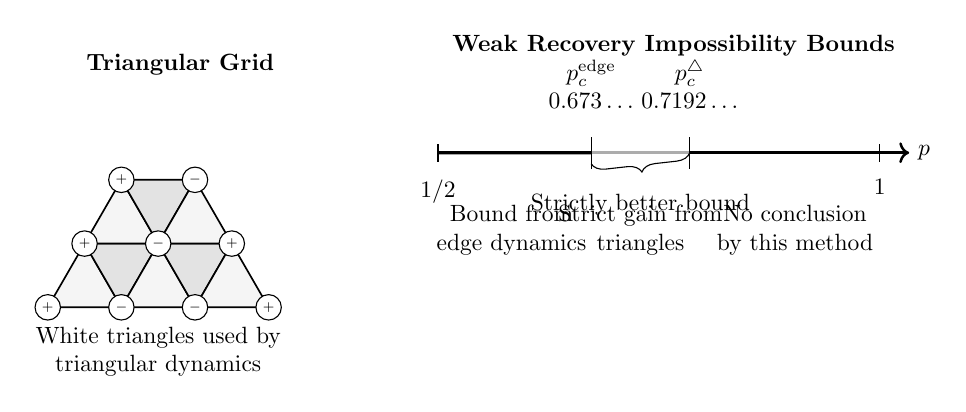
\begin{tikzpicture}[x=1.1cm,y=1.1cm, scale=0.85, every node/.style={scale=0.85}]
      % triangular grid left
      \begin{scope}[shift={(0,0.5)}]
        \node at (1.8,3.3) {\textbf{Triangular Grid}};
        \coordinate (a) at (0,0); \coordinate (b) at (1,0); \coordinate (c) at (2,0); \coordinate (d) at (3,0);
        \coordinate (e) at (.5,.866); \coordinate (f) at (1.5,.866); \coordinate (g) at (2.5,.866);
        \coordinate (h) at (1,1.732); \coordinate (i) at (2,1.732);
        \filldraw[triwhite] (a)--(b)--(e)--cycle;
        \filldraw[trigray] (b)--(e)--(f)--cycle;
        \filldraw[triwhite] (b)--(c)--(f)--cycle;
        \filldraw[trigray] (c)--(f)--(g)--cycle;
        \filldraw[triwhite] (c)--(d)--(g)--cycle;
        \filldraw[triwhite] (e)--(f)--(h)--cycle;
        \filldraw[trigray] (f)--(h)--(i)--cycle;
        \filldraw[triwhite] (f)--(g)--(i)--cycle;
        \foreach \p/\s in {a/+,b/-,c/-,d/+,e/+,f/-,g/+,h/+,i/-}
          \node[tinynode] at (\p) {$\s$};
        \node[align=center] at (1.5,-0.6) {White triangles used by\\triangular dynamics};
      \end{scope}

      % number line right
      \begin{scope}[shift={(5.3,1.0)}]
        \node at (3.2,3.05) {\textbf{Weak Recovery Impossibility Bounds}};
        \draw[->,line width=.9pt] (0,1.6)--(6.4,1.6) node[right] {$p$};
        \draw (0,1.48)--(0,1.72) node[below=.35cm] {$1/2$};
        \draw (6,1.48)--(6,1.72) node[below=.35cm] {$1$};
        \coordinate (pe) at (2.08,1.6);
        \coordinate (pt) at (3.42,1.6);
        \draw[very thick] (0,1.6)--(pe);
        \draw[very thick,gray!65] (pe)--(pt);
        \draw[dashed] (pt)--(6,1.6);
        \draw (pe)+(0,-.22)--+(0,.22) node[above=.25cm,align=center] {$p_c^{\mathrm{edge}}$\\$0.673\ldots$};
        \draw (pt)+(0,-.22)--+(0,.22) node[above=.25cm,align=center] {$p_c^{\triangle}$\\$0.7192\ldots$};
        \node[align=center] at (1.0,.55) {Bound from\\edge dynamics};
        \node[align=center] at (2.75,.55) {Strict gain from\\triangles};
        \node[align=center] at (4.85,.55) {No conclusion\\by this method};
        \draw[decorate,decoration={brace,mirror,amplitude=5pt}] (pe)+(0,-0.15)--(pt)+(0,-0.15) node[midway,below=.35cm] {Strictly better bound};
      \end{scope}
    \end{tikzpicture}
  \end{figure}
\end{frame}

%%%%%%%%%%%%%%%%%%%%%%%%%%%%%%%%%%%%%%%%%%%%%%%%%%%%%%%
\section{Open Questions \& Conclusion}
\frame{\sectionpage}

\begin{frame}{Open Questions}
  \begin{block}{1. Extension to Other Lattices and Higher Dimensions}
    \begin{itemize}
      \item What are the thresholds on the Kagome, FCC, HCP, or Hyper-cubic lattices?
      \item Can we define tetrahedral or higher-order simplex dynamics to obtain even tighter bounds?
    \end{itemize}
  \end{block}
  \begin{block}{2. Multi-Community case ($K > 2$)}
    \begin{itemize}
      \item How does the cluster dynamics extend when the spins take $K$ values?
      \item What is the role of \textsc{Potts}-like percolation in the coupling?
    \end{itemize}
  \end{block}
  \begin{block}{3. Sufficiency of the Percolation Condition}
    \begin{itemize}
      \item The percolation threshold provides a necessary condition (impossibility).
      \item Is percolation also sufficient for the existence of a reconstruction algorithm?
    \end{itemize}
  \end{block}
\end{frame}

\begin{frame}[allowframebreaks]{Bibliography}
  \printbibliography
\end{frame}

\frame{\merci}

\end{document}
